\documentclass[12pt]{article}
\usepackage[left=0.5in,right=0.5in,top=0.5in,left=0.5in]{geometry}
\usepackage{algpseudocode}
\usepackage{algorithm}
\usepackage{circuitikz}
\usepackage{amsfonts}
\usepackage{amsmath}

\title{\textsc{Homework 1}}
\author{Henry Trinh}

\begin{document}
\maketitle

\newpage % PROBLEM 1 %
\section*{Problem 1}
\subsection*{Part A}
$\forall (n, k \in \mathbb{N}), \phi(n,k) = \exists a \in \mathbb{N} (a * k = n)$
\subsection*{Part B}
$\forall (n, k \in \mathbb{N}), \phi(n) = \exists a \in \mathbb{N} (3^a = n)$

\newpage
\section*{Problem 2}
\subsection*{Part A}
$F=O(G)$
\newline
\newline
$F$ and $G$ have the same polynomial factor of linear time. Furthermore, if you take the limit 
of $F/G$, the limit will be a constant number.
\subsection*{Part B}
$F=\omega(G)$
\newline
\newline
F has a polynomial factor of 1 while G only has a polynomial factor of 0.5, so 
F will grow at a much faster rate. If we take the limit of $F/G$, it will be equal 
to infinity.
\subsection*{Part C}
$F=o(G)$
\newline
\newline
Since G is an exponential function, it will grow at a much faster rate than F since it is in the magnitude of 
$nlogn$.
\newline
\newline
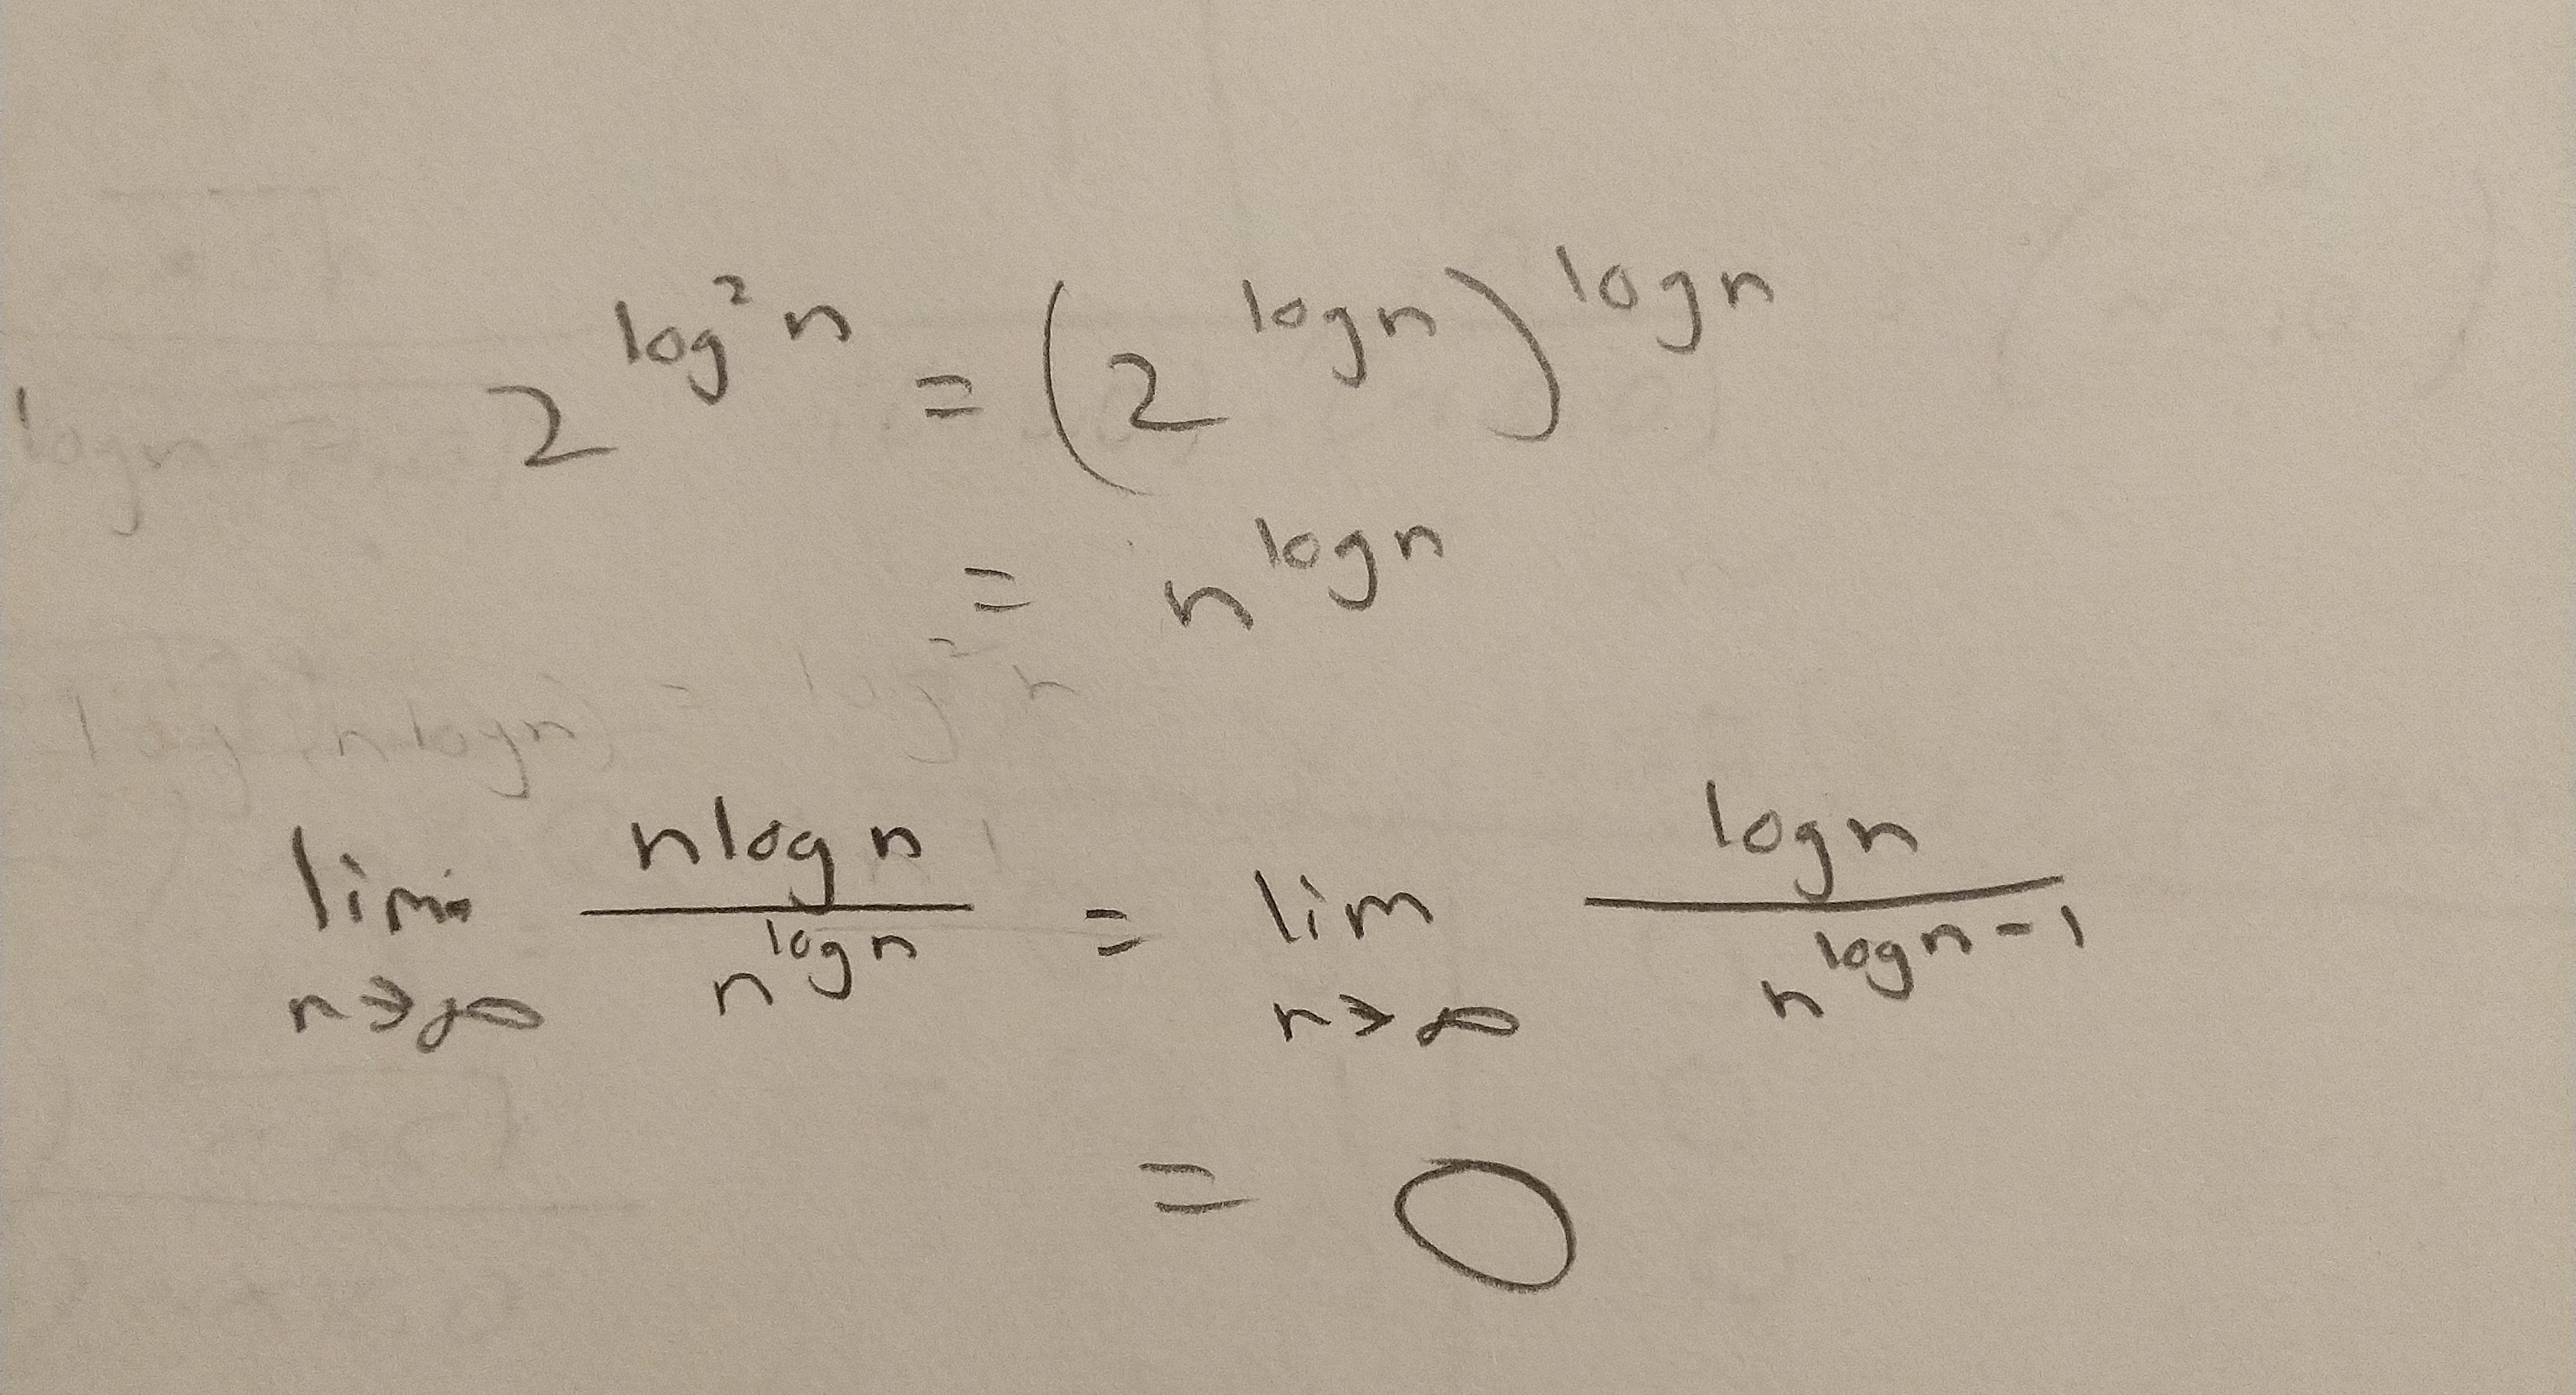
\includegraphics[scale=0.1, angle=0]{problem2c.jpeg}
\newline
\subsection*{Part D}
$F=o(G)$
\newline
\newline
Since exponential functions grow at a much faster rate than polynomial functions, we can
deduce that the limit of $F/G$ goes to 0 since $F$ is polynomial and $G$ is exponential.
\subsection*{Part E}
$F=\omega(G)$
\newline
\newline
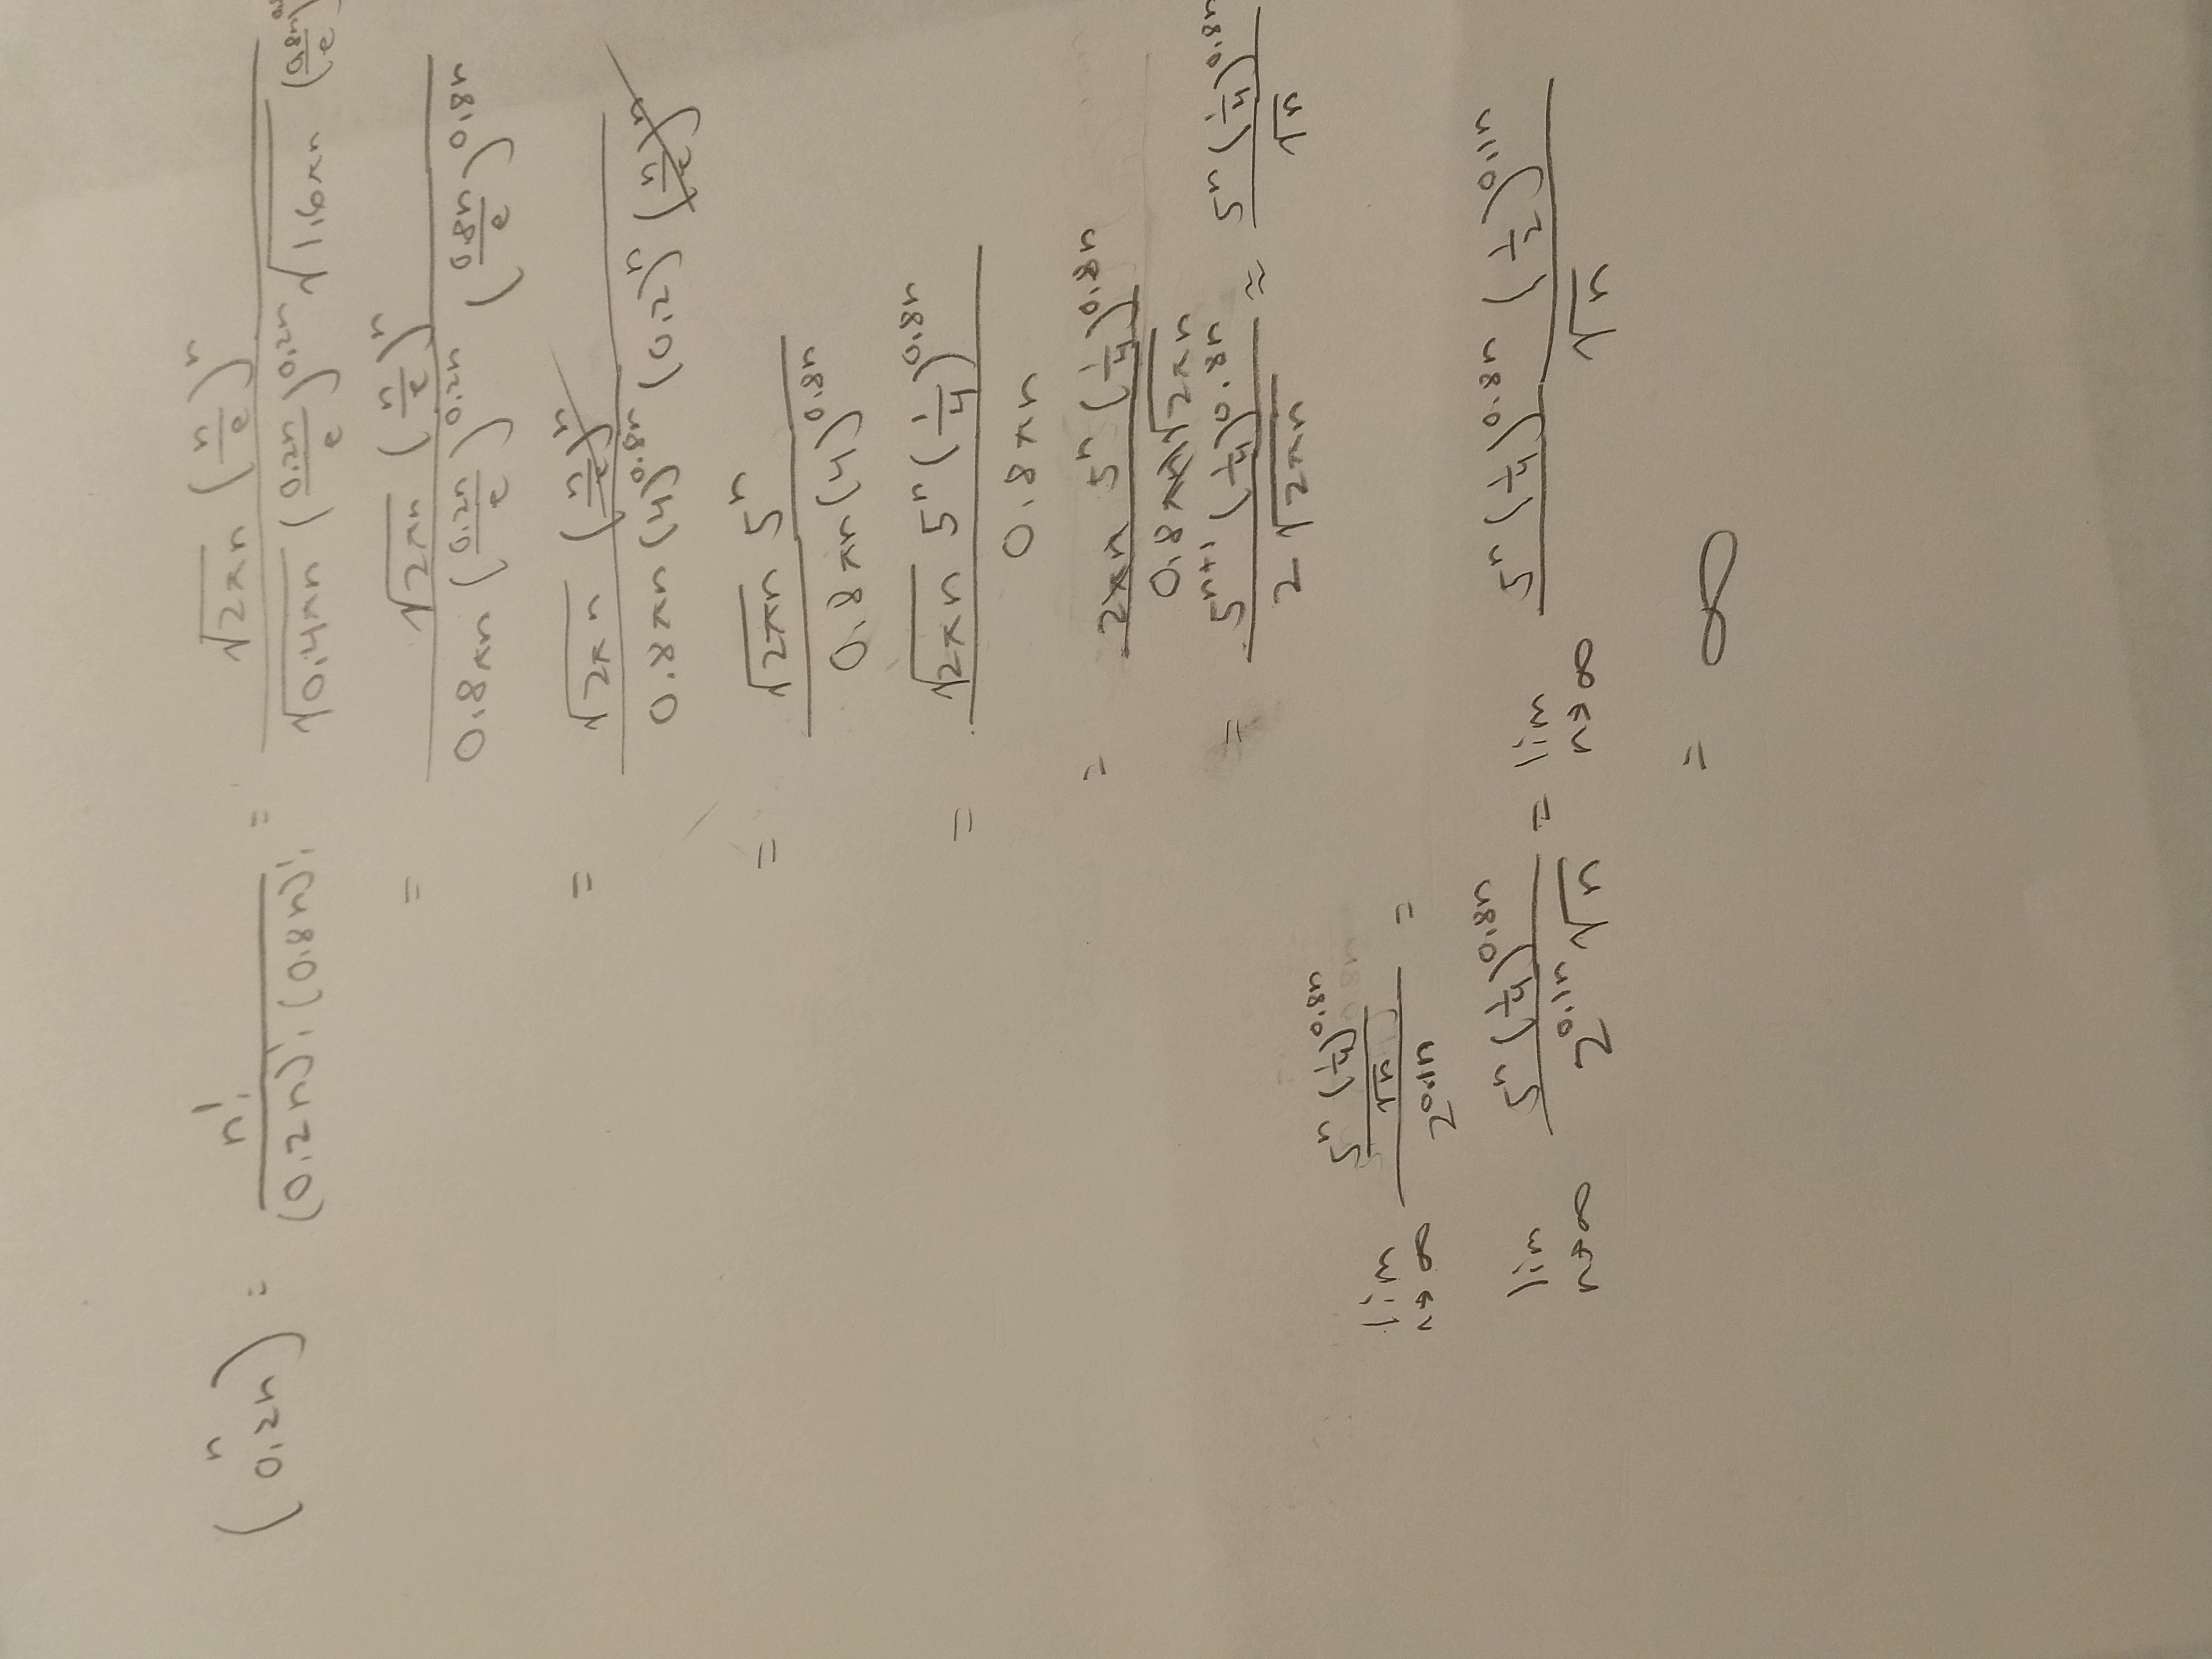
\includegraphics[scale=0.1, angle=-90]{problem2e.jpg}

\newpage
\section*{Problem 3}
Given sets $S$ and $T$, assume that $|S| > |T|$ and that there is a one-to-one mapping from $S$ to $T$.
This means that for every element in $S$, it will be paired with its own unique element from $T$. 
However, by the pigeonhole principle, there will be elements in $S$ that will be paired with the 
same element in $T$ because there are more elements in $S$ than $T$. However, this observation
is a direct contradiction to our given that there is a one-to-one mapping from $S$ to $T$. This shows
that there is only a one-to-one mapping from $S$ to $T$ if and only if $|S| \leq |T|$.

\newpage
\section*{Problem 4}
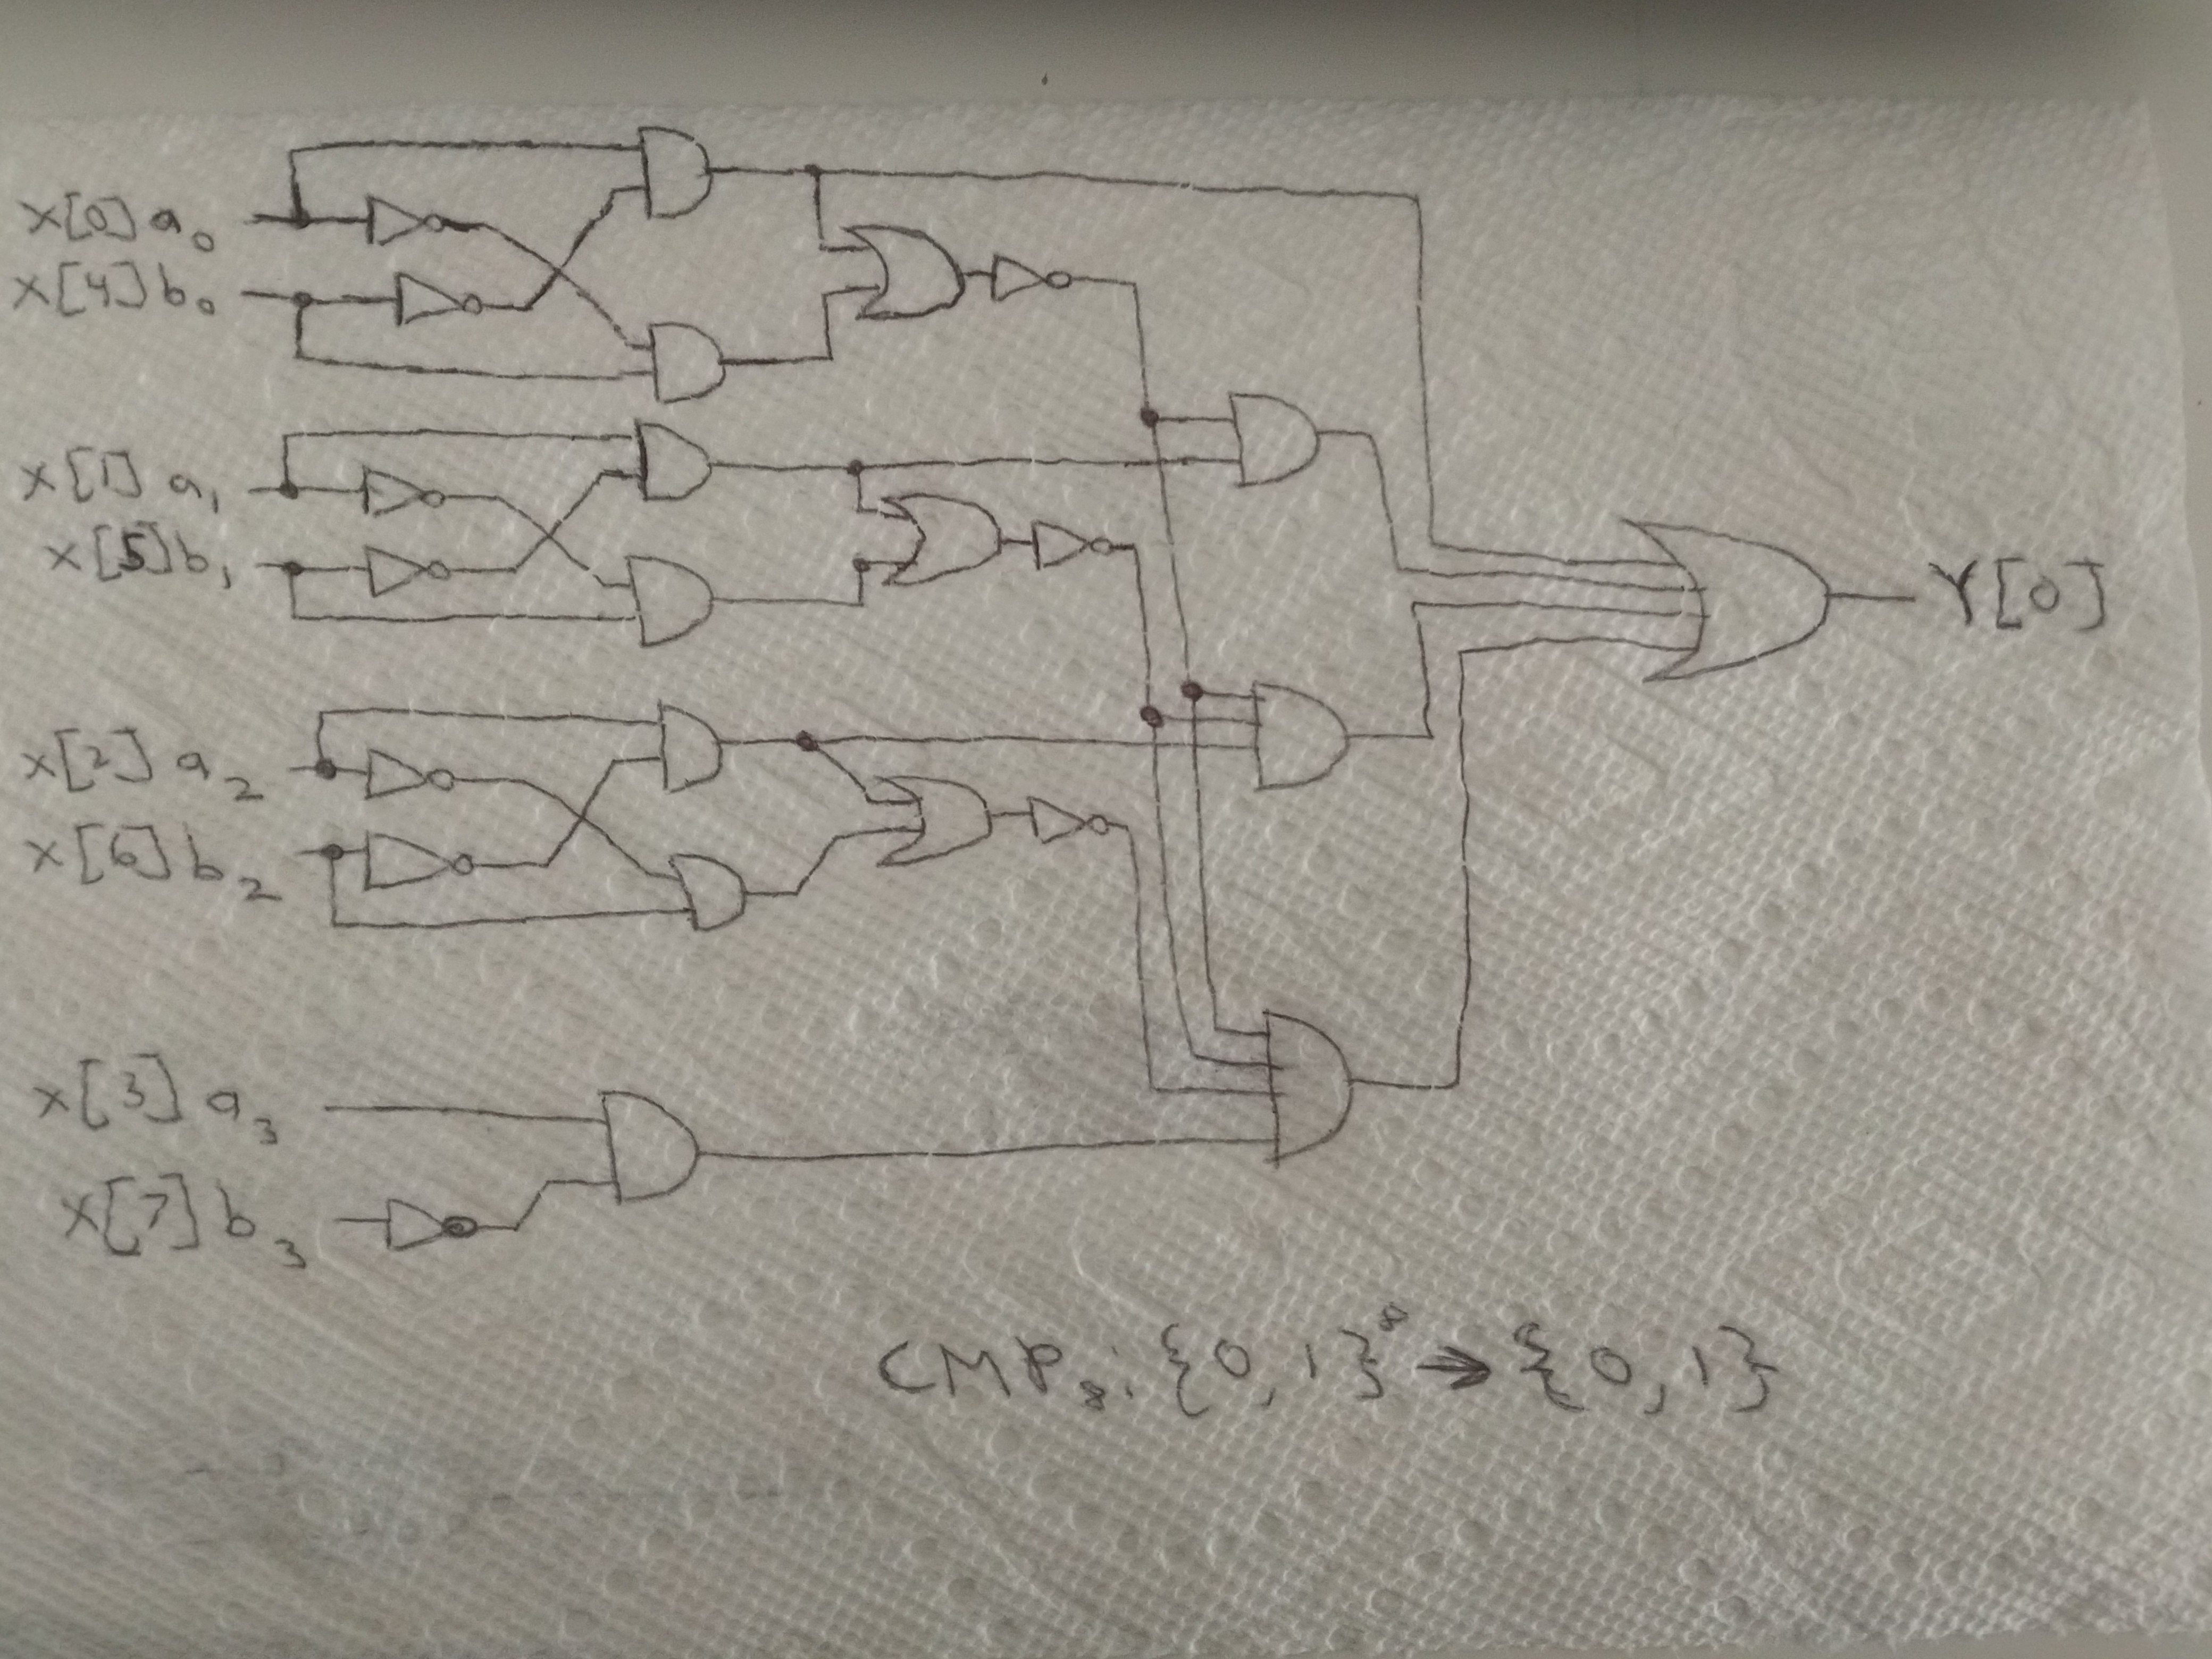
\includegraphics[scale=0.15, angle=-90]{problem4.jpg}

\newpage
\section*{Problem 5}
The set of the gates \{AND, OR, 0, 1\} is not universal because this set is strictly monotonically increasing.
For every gate in the set \{AND, OR, 0, 1\} represented as $f$, given an input $a\in \mathbb{N}$ and $b\in \mathbb{N}$ 
such that $a < b$, then $f(a) \leq f(b)$. Since all these gates have this property, they are all monotonically increasing.
If we create a boolean circuit using only gates from the set \{AND, OR, 0, 1\}, the output will always
follow the pattern of monotonically increasing outputs for any input given similar to the individual gates. 
Since for any combination of the gates in \{AND, OR, 0, 1\}, we cannot produce an output of $f(a) \geq f(b)$ where
$a < b$ and thus we cannot create any circuit that is non-increasing. Therefore, \{AND, OR, 0, 1\} is not universal.

\newpage
\section*{Problem 6}
We can prove that \{LOOKUP, 0, 1\} is a universal set of gates by showing that we can recreate another known
universal set of gates, \{AND, OR, NOT\}, using \{LOOKUP, 0, 1\}. We can show this by doing so:
\newline
\newline
$NOT(x) = LOOKUP(1, 0, x)$
\newline
$AND(x, y) = LOOKUP(0, y, x)$
\newline
$OR(x, y)=LOOKUP(y, 1, x)$
\newline
\newline
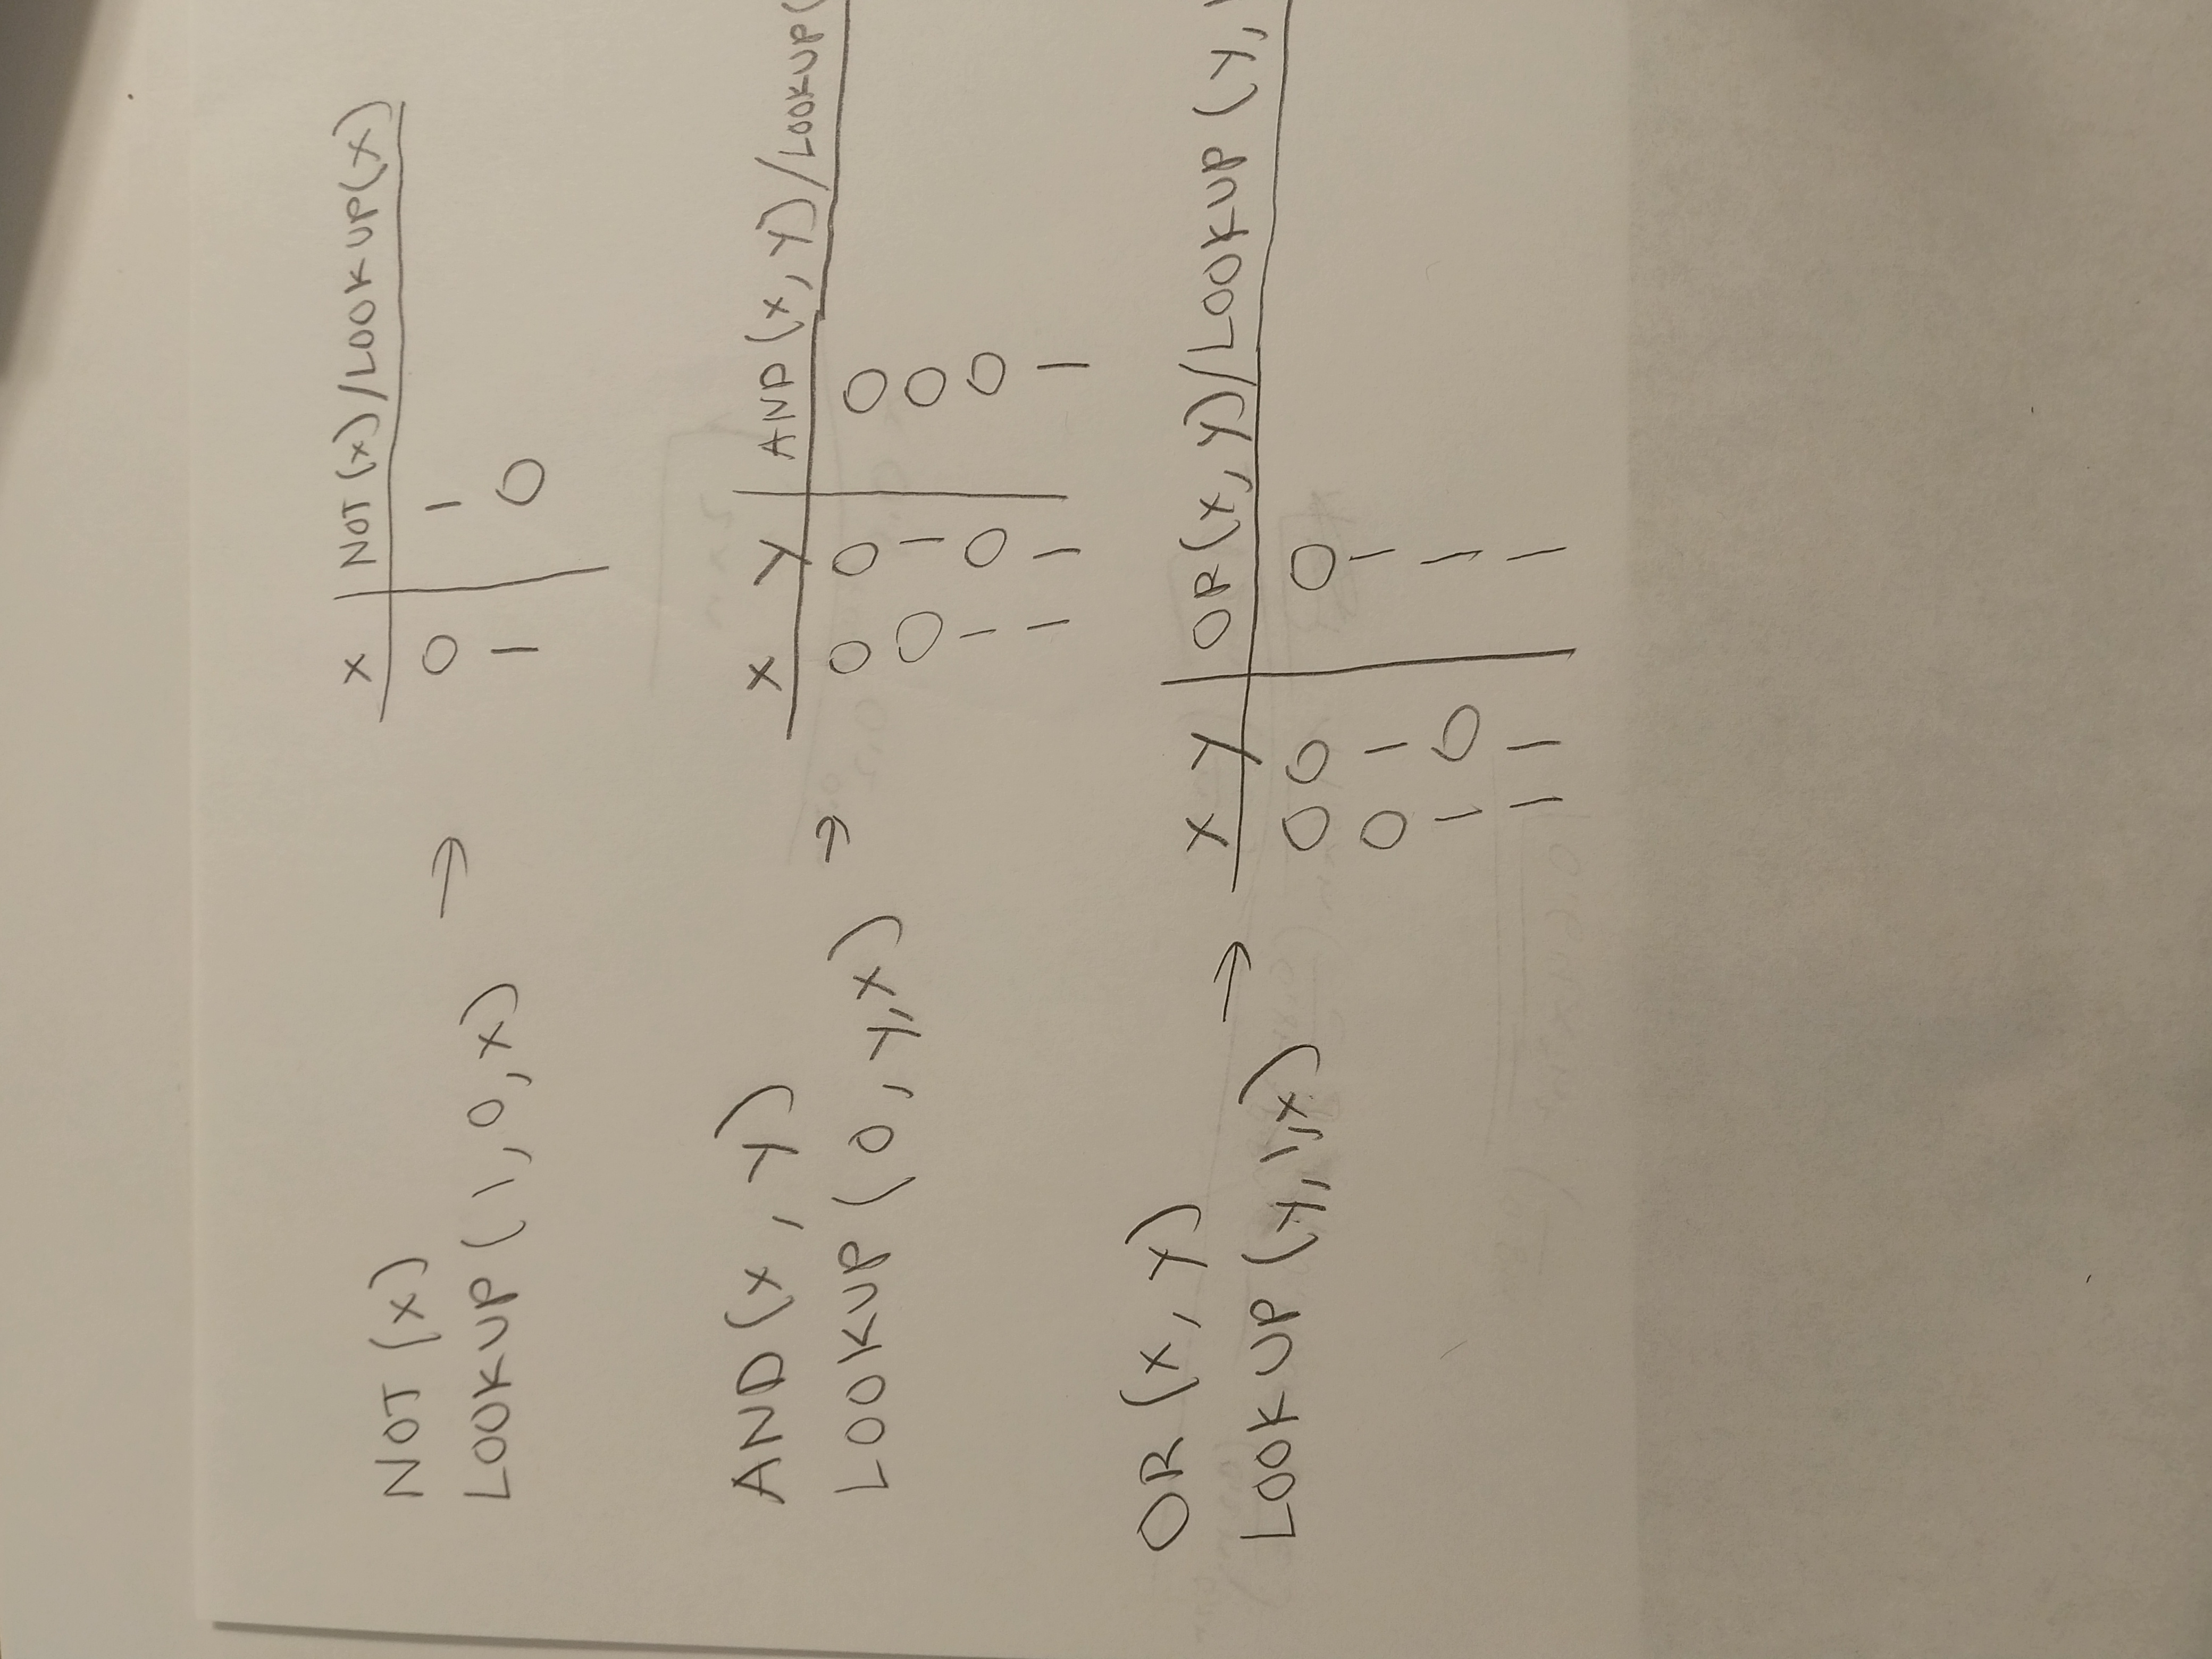
\includegraphics[scale=0.08, angle=-90]{problem6.jpg}
\newline
\newline
Since we can recreate the universal set \{NOT, AND, OR\} using the set \{LOOKUP, 0, 1\}, we can conclude that
\{LOOKUP, 0, 1\} is also a universal set.



\end{document}